\section*{Results of the final optimized run}

The final protocol uses only paths of 1,000 events, with 75,000 training
samples, 10,000 validation samples and 15,000 test samples.
The networks are summarized over five independent seeds; the MLE is fitted
separately on each path of the same test set.
The network intervals use Student's $t$ distribution across seeds.

\begin{table}[htbp]
\centering
\caption{Aggregate metrics on the frozen synthetic test set (15,000 paths of 1,000 events).}
\label{tab:final-agregado}
\small
\begin{tabular}{lrrrrr}
\toprule
Estimator & Macro MSE & 95\% CI & Macro MAE & MSE of $g$ & Validity\\
\midrule
LSTM & 0.019618 & [0.013252, 0.025984] & 0.094276 & 0.001825 & 100.00\%\\
Transformer & 0.023700 & [0.019128, 0.028272] & 0.105642 & 0.002138 & 100.00\%\\
MLE & 0.506193 & -- & 0.111852 & 0.002344 & 100.00\%\\
\bottomrule
\end{tabular}
\end{table}

\begin{table}[htbp]
\centering
\caption{Test MSE by parameter (networks: mean over five seeds).}
\label{tab:final-parametros}
\begin{tabular}{lrrrr}
\toprule
Estimator & $\mu$ & $\alpha_{\mathrm{self}}$ & $\alpha_{\mathrm{cross}}$ & $\beta$\\
\midrule
LSTM & 0.002296 & 0.016222 & 0.016566 & 0.043386\\
Transformer & 0.002366 & 0.020905 & 0.021196 & 0.050332\\
MLE & 0.010108 & 0.006146 & 0.006214 & 2.002303\\
\bottomrule
\end{tabular}
\end{table}

\begin{table}[htbp]
\centering
\caption{Macro MSE by regime of the branching ratio $g$.}
\label{tab:final-regimes}
\begin{tabular}{lrrr}
\toprule
Estimator & Low $g$ & Intermediate $g$ & Near-critical $g$\\
\midrule
LSTM & 0.019941 & 0.015614 & 0.023297\\
Transformer & 0.022228 & 0.018964 & 0.029908\\
MLE & 1.480568 & 0.016795 & 0.021214\\
\bottomrule
\end{tabular}
\end{table}

Between the networks, the LSTM obtained a mean macro MSE 17.2\% lower than the Transformer.
With 5 and 5 seeds, however, the difference is not statistically significant (Welch test, $p=0.19$), and the confidence intervals overlap; the data do not allow the networks to be ranked.
For the MLE, the parameter $\beta$ accounted for 98.9\% of the sum of
squared errors, and the macro MSE in the low-$g$ regime was 88.15 times
that of the intermediate regime: with weak excitation, $\beta$ is weakly
identified and some paths produce extreme estimates. Outside this regime the
MLE is competitive: in the intermediate regime its macro MSE was 0.0168 (LSTM:
0.0156; Transformer: 0.0190) and, in the near-critical regime,
0.0212 (LSTM: 0.0233; Transformer: 0.0299).
The MLE obtained the lowest MSE among the three estimators for $\alpha_{\mathrm{self}}$ and $\alpha_{\mathrm{cross}}$.
Therefore, the aggregate macro MSE does not rank the estimators robustly,
and numerical convergence does not imply good parameter recovery.

\begin{figure}[htbp]
\centering
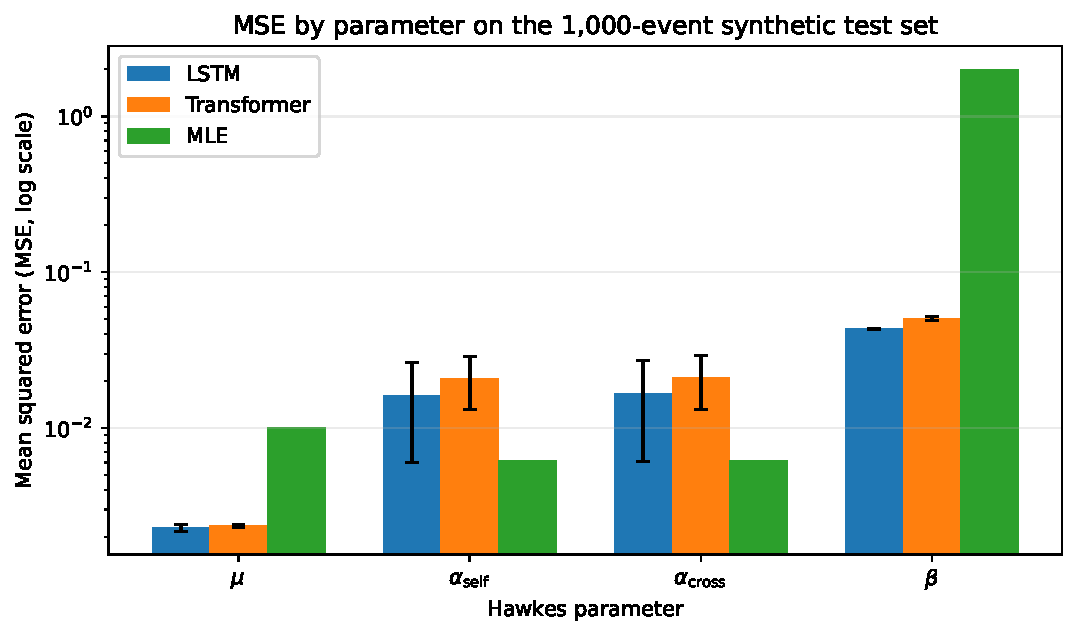
\includegraphics[width=0.88\linewidth]{../build/figures/parameter_mse_en.pdf}
\caption{Test MSE by parameter under the 1,000-event protocol.
The network error bars represent one standard deviation across seeds.}
\end{figure}

\begin{figure}[htbp]
\centering
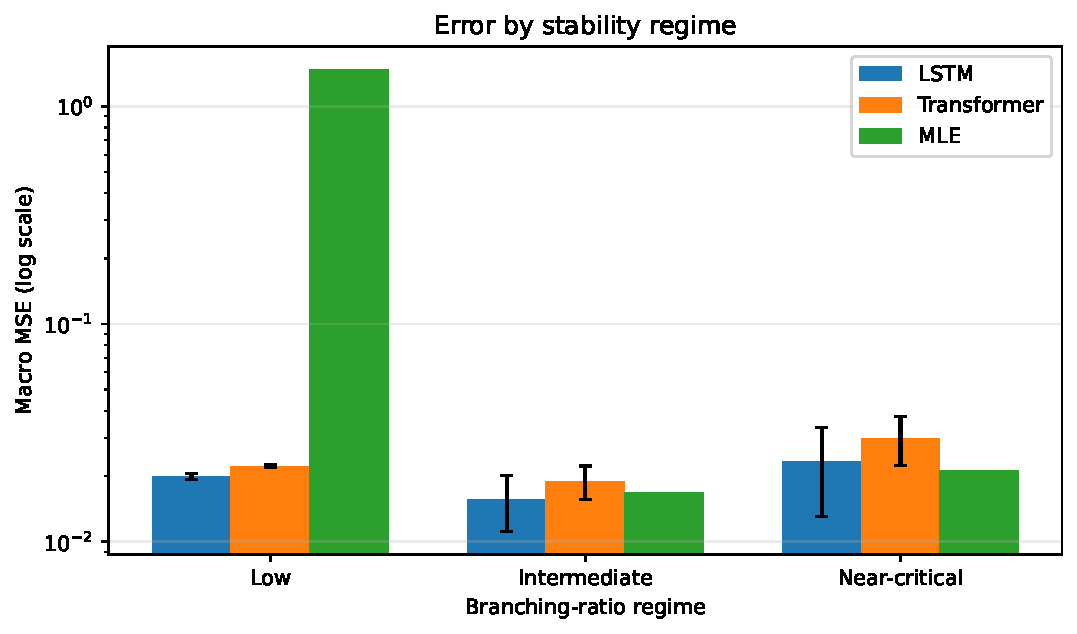
\includegraphics[width=0.88\linewidth]{../build/figures/branching_regime_mse_en.pdf}
\caption{Macro MSE by regime of the branching ratio. The network error
bars represent one standard deviation across seeds.}
\end{figure}

\begin{figure}[htbp]
\centering
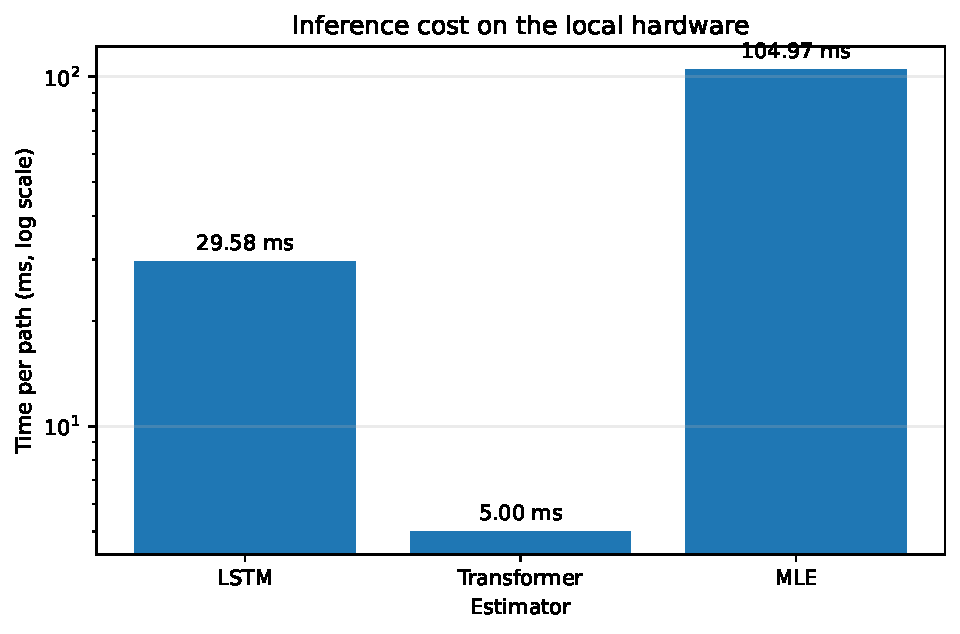
\includegraphics[width=0.80\linewidth]{../build/figures/inference_cost_en.pdf}
\caption{Cost per path recorded during the final run, on a logarithmic
scale. For the MLE, wall-clock time with four processes competing with
training on the GPU; for the networks, median latency at batch size one on
MPS. A later controlled benchmark measured about 10~ms per path for the MLE
on a single core and should be preferred to this figure.}
\end{figure}

The MLE converged on 100.00\% of the paths
and used a median of 14.00 iterations.
All comparisons use the same frozen test set.
